\section{Problem 2}

\subsection{Introduction}

This report presents a comprehensive data analysis workflow applied to the dataset \texttt{e6-Run2-June22-subset-100-cols.csv}. The main objectives include data cleaning, outlier detection, normalization, correlation analysis, multicollinearity assessment, and Principal Component Analysis (PCA).

\subsection{Methodology}

\subsubsection{Data Loading and Initial Exploration}
The data was loaded using the \texttt{pandas} library. Initial exploration was performed to understand the structure and quality of the data.

\begin{lstlisting}[language=Python]
import pandas as pd
import numpy as np
import seaborn as sns
import matplotlib.pyplot as plt

df = pd.read_csv('e6-Run2-June22-subset-100-cols.csv')
print(df.head(10))
print(df.describe())
print(df.isnull().sum())
\end{lstlisting}

\subsubsection{Data Cleaning}
Data cleaning involved the following steps:

\begin{itemize}
    \item **Column Retention:** Columns with low variance were dropped based on a variance threshold of 0.05.
    \item **Handling Missing Values:** Missing values were replaced with the mean of each column.
    \item **Outlier Detection:** Outliers were detected using the Interquartile Range (IQR) method, and appropriate action was taken.
\end{itemize}

\begin{lstlisting}[language=Python]
# Step 1: Replace non-numeric values
df.replace('#REF!', np.nan, inplace=True)

# Step 2: Drop low variance columns
variances = df.var()
low_variance_columns = variances[variances < 0.05].index
df.drop(columns=low_variance_columns, inplace=True)

# Step 3: Handle missing values
df.fillna(df.mean(), inplace=True)

# Step 4: Outlier detection using IQR
Q1 = df.quantile(0.25)
Q3 = df.quantile(0.75)
IQR = Q3 - Q1
outlier_condition = (df < (Q1 - 1.5 * IQR)) | (df > (Q3 + 1.5 * IQR))
df = df[~outlier_condition.any(axis=1)]
\end{lstlisting}

\subsubsection{Normalization}
Standardization was performed on the numeric columns to prepare the data for PCA.

\begin{lstlisting}[language=Python]
from sklearn.preprocessing import StandardScaler
scaler = StandardScaler()
df_scaled = pd.DataFrame(scaler.fit_transform(df), columns=df.columns)
\end{lstlisting}

\subsubsection{Correlation Analysis}
A correlation matrix was computed and visualized to identify highly correlated features.

\begin{lstlisting}[language=Python]
corr_matrix = df_scaled.corr()
plt.figure(figsize=(12, 10))
sns.heatmap(corr_matrix, annot=True, fmt=".2f", cmap='RdBu_r', square=True)
plt.title("Correlation Heatmap")
plt.show()
\end{lstlisting}

\begin{figure}[H]
    \centering
    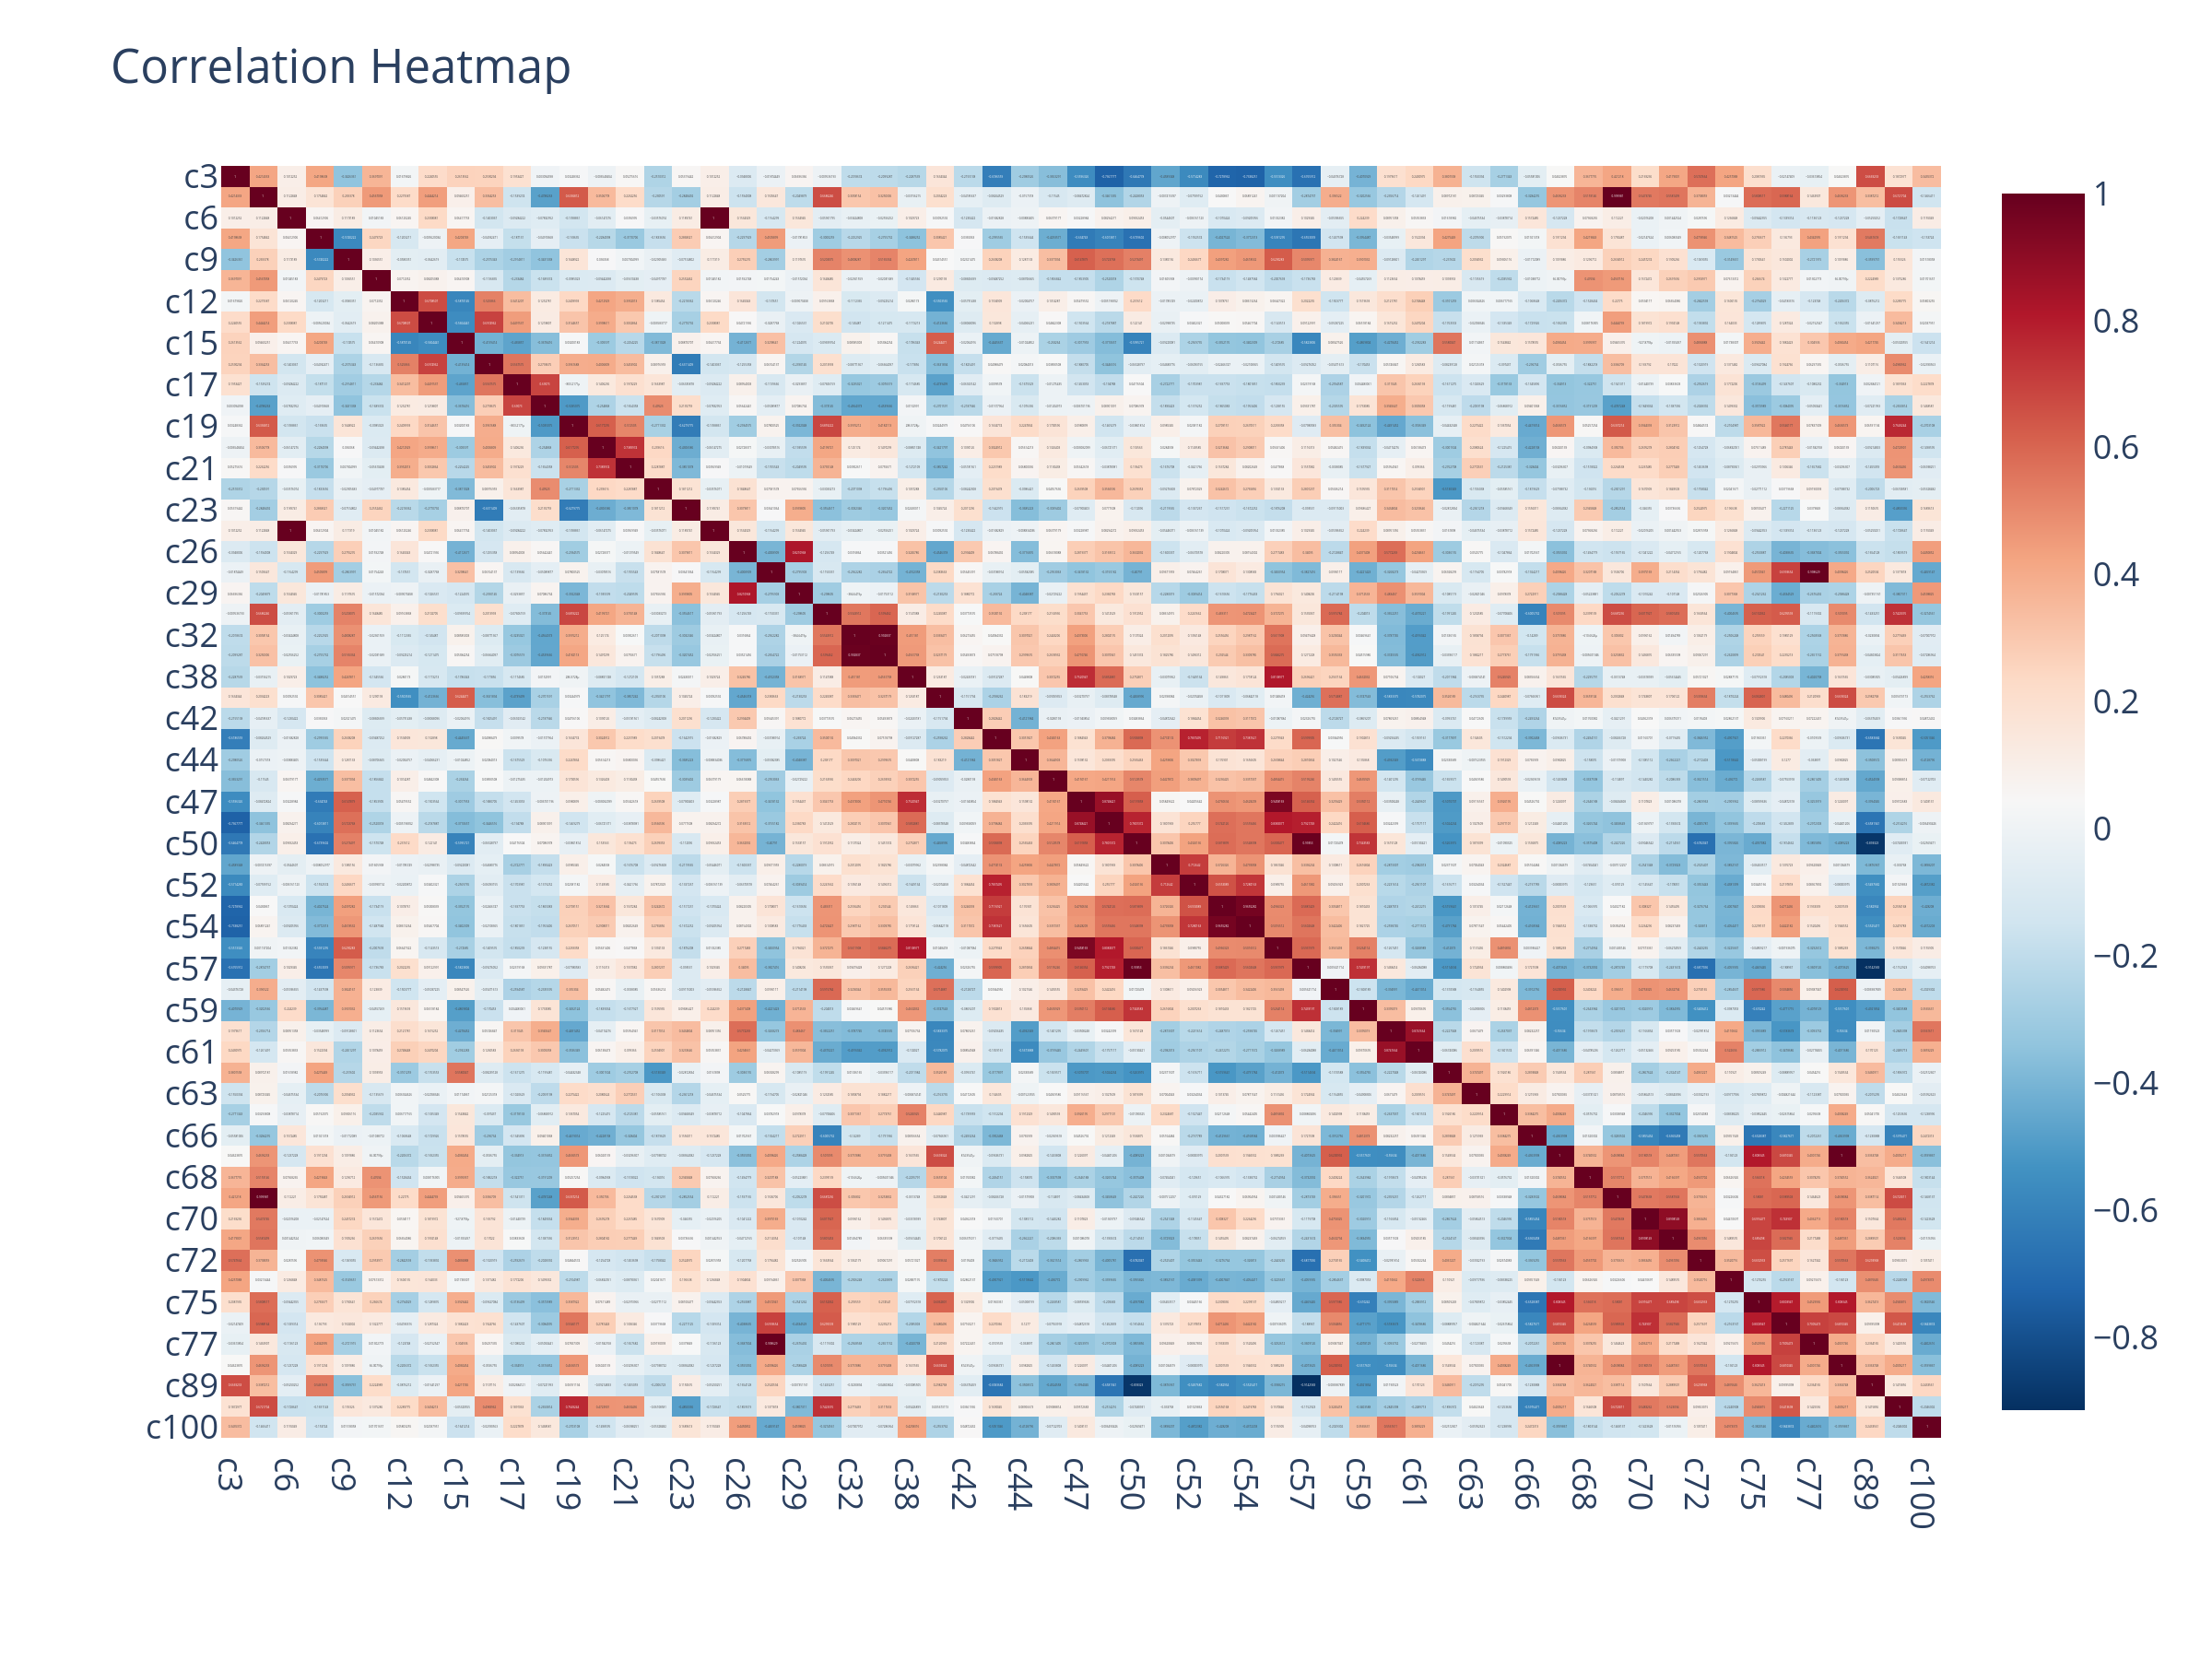
\includegraphics[width=0.6\textwidth]{Images/correlation_heatmap.png}
    \caption{Correlation Heatmap}
\end{figure}


\subsubsection{Multicollinearity Assessment}
Variance Inflation Factor (VIF) was calculated to identify multicollinearity among features.

\begin{lstlisting}[language=Python]
from statsmodels.stats.outliers_influence import variance_inflation_factor

vif_data = pd.DataFrame()
vif_data["feature"] = df_scaled.columns
vif_data["VIF"] = [variance_inflation_factor(df_scaled.values, i) for i in range(len(df_scaled.columns))]
print(vif_data)
\end{lstlisting}

\subsubsection{Dealing with Correlated Columns}
Based on the correlation and VIF analysis, columns with high correlation (greater than 0.8) or high VIF values (greater than 10) were identified and removed.

\begin{lstlisting}[language=Python]
# Dropping correlated columns based on threshold
corr_threshold = 0.8
columns_to_drop = set()

for i in range(len(corr_matrix.columns)):
    for j in range(i):
        if abs(corr_matrix.iloc[i, j]) > corr_threshold:
            colname = corr_matrix.columns[i]
            columns_to_drop.add(colname)

df_scaled.drop(columns=columns_to_drop, inplace=True)
\end{lstlisting}

\subsubsection{Principal Component Analysis (PCA)}
PCA was conducted to reduce the dimensionality of the dataset, both before and after addressing multicollinearity. Elbow diagrams were generated to visualize cumulative explained variance.

\begin{lstlisting}[language=Python]
from sklearn.decomposition import PCA

# PCA before removing correlated features
pca_initial = PCA()
df_pca_initial = pca_initial.fit_transform(df_scaled)
explained_variance_initial = pca_initial.explained_variance_ratio_

# PCA after removing correlated features
pca_final = PCA()
df_pca_final = pca_final.fit_transform(df_scaled)
explained_variance_final = pca_final.explained_variance_ratio_

# Cumulative explained variance
cumulative_variance_initial = np.cumsum(explained_variance_initial)
cumulative_variance_final = np.cumsum(explained_variance_final)
\end{lstlisting}

\subsubsection{Elbow Diagram Creation}
Elbow diagrams were plotted to visualize the explained variance.

\begin{lstlisting}[language=Python]
# Elbow Diagram before removing correlated features
plt.figure(figsize=(12, 6))
plt.plot(range(1, len(cumulative_variance_initial) + 1), cumulative_variance_initial, marker='o')
plt.title('Elbow Diagram (Before Removing Correlated Features)')
plt.xlabel('Number of Components')
plt.ylabel('Cumulative Explained Variance')
plt.grid()
plt.show()

# Elbow Diagram after removing correlated features
plt.figure(figsize=(12, 6))
plt.plot(range(1, len(cumulative_variance_final) + 1), cumulative_variance_final, marker='o', color='orange')
plt.title('Elbow Diagram (After Removing Correlated Features)')
plt.xlabel('Number of Components')
plt.ylabel('Cumulative Explained Variance')
plt.grid()
plt.show()
\end{lstlisting}

\subsection{Results}

\subsubsection{Data Cleaning Results}
The cleaning process resulted in the removal of columns with low variance and handling of missing values. The number of columns dropped due to low variance was \texttt{len(low\_variance\_columns)}.

\subsubsection{Correlation Analysis Results}
The correlation heatmap indicated the presence of highly correlated features. A total of \texttt{len(columns\_to\_drop)} columns were dropped due to high correlation.

% \subsubsection{VIF Analysis Results}
% The VIF analysis showed the following features with high VIF values:
% \begin{center}
% \begin{tabular}{l c}
% \toprule
% Feature & VIF \\
% \midrule
% % Insert VIF results here
% \bottomrule
% \end{tabular}
% \end{center}

\subsubsection{PCA Results}
The PCA results showed that the optimal number of components explaining at least 95\% of the variance was determined. The cumulative variance explained for the initial and final PCA were \texttt{explained\_variance\_initial} and \texttt{explained\_variance\_final} respectively.

\begin{figure}[H]
    \centering
    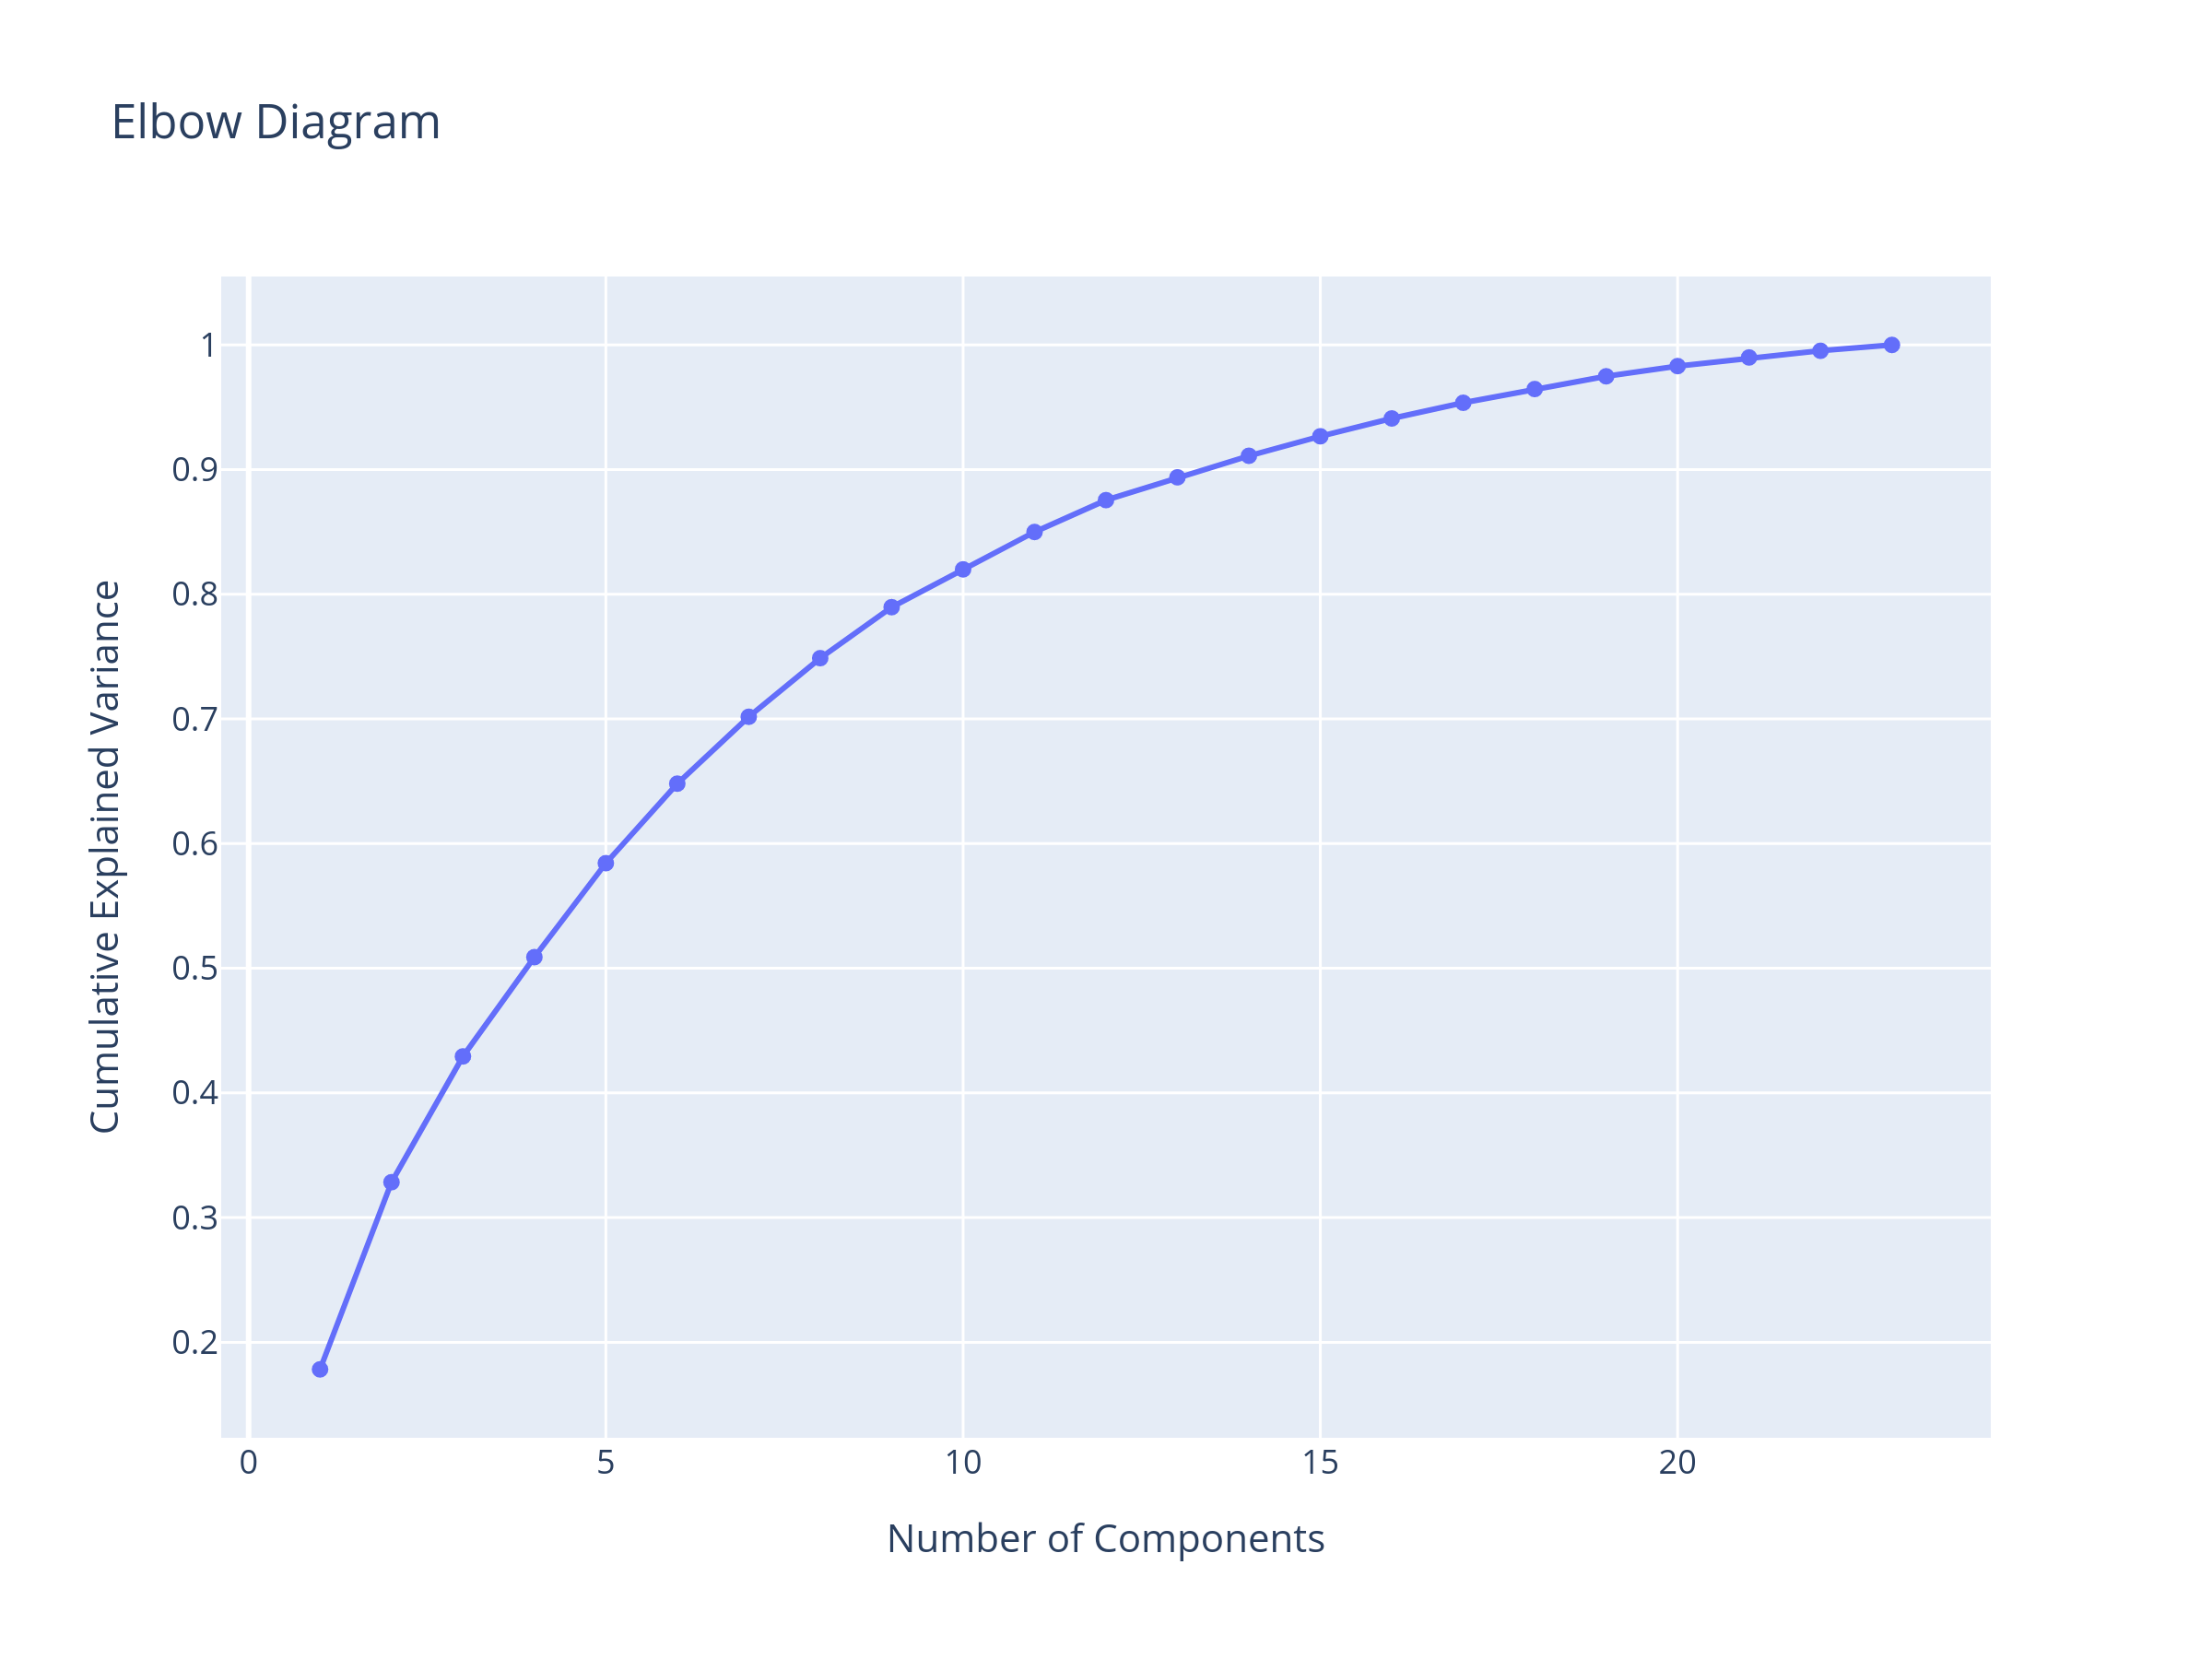
\includegraphics[width=0.6\textwidth]{Images/elbow_diagram_before_vif.png}
    \caption{Elbow Diagram (Before Removing Correlated Features)}
\end{figure}

\begin{figure}[H]
    \centering
    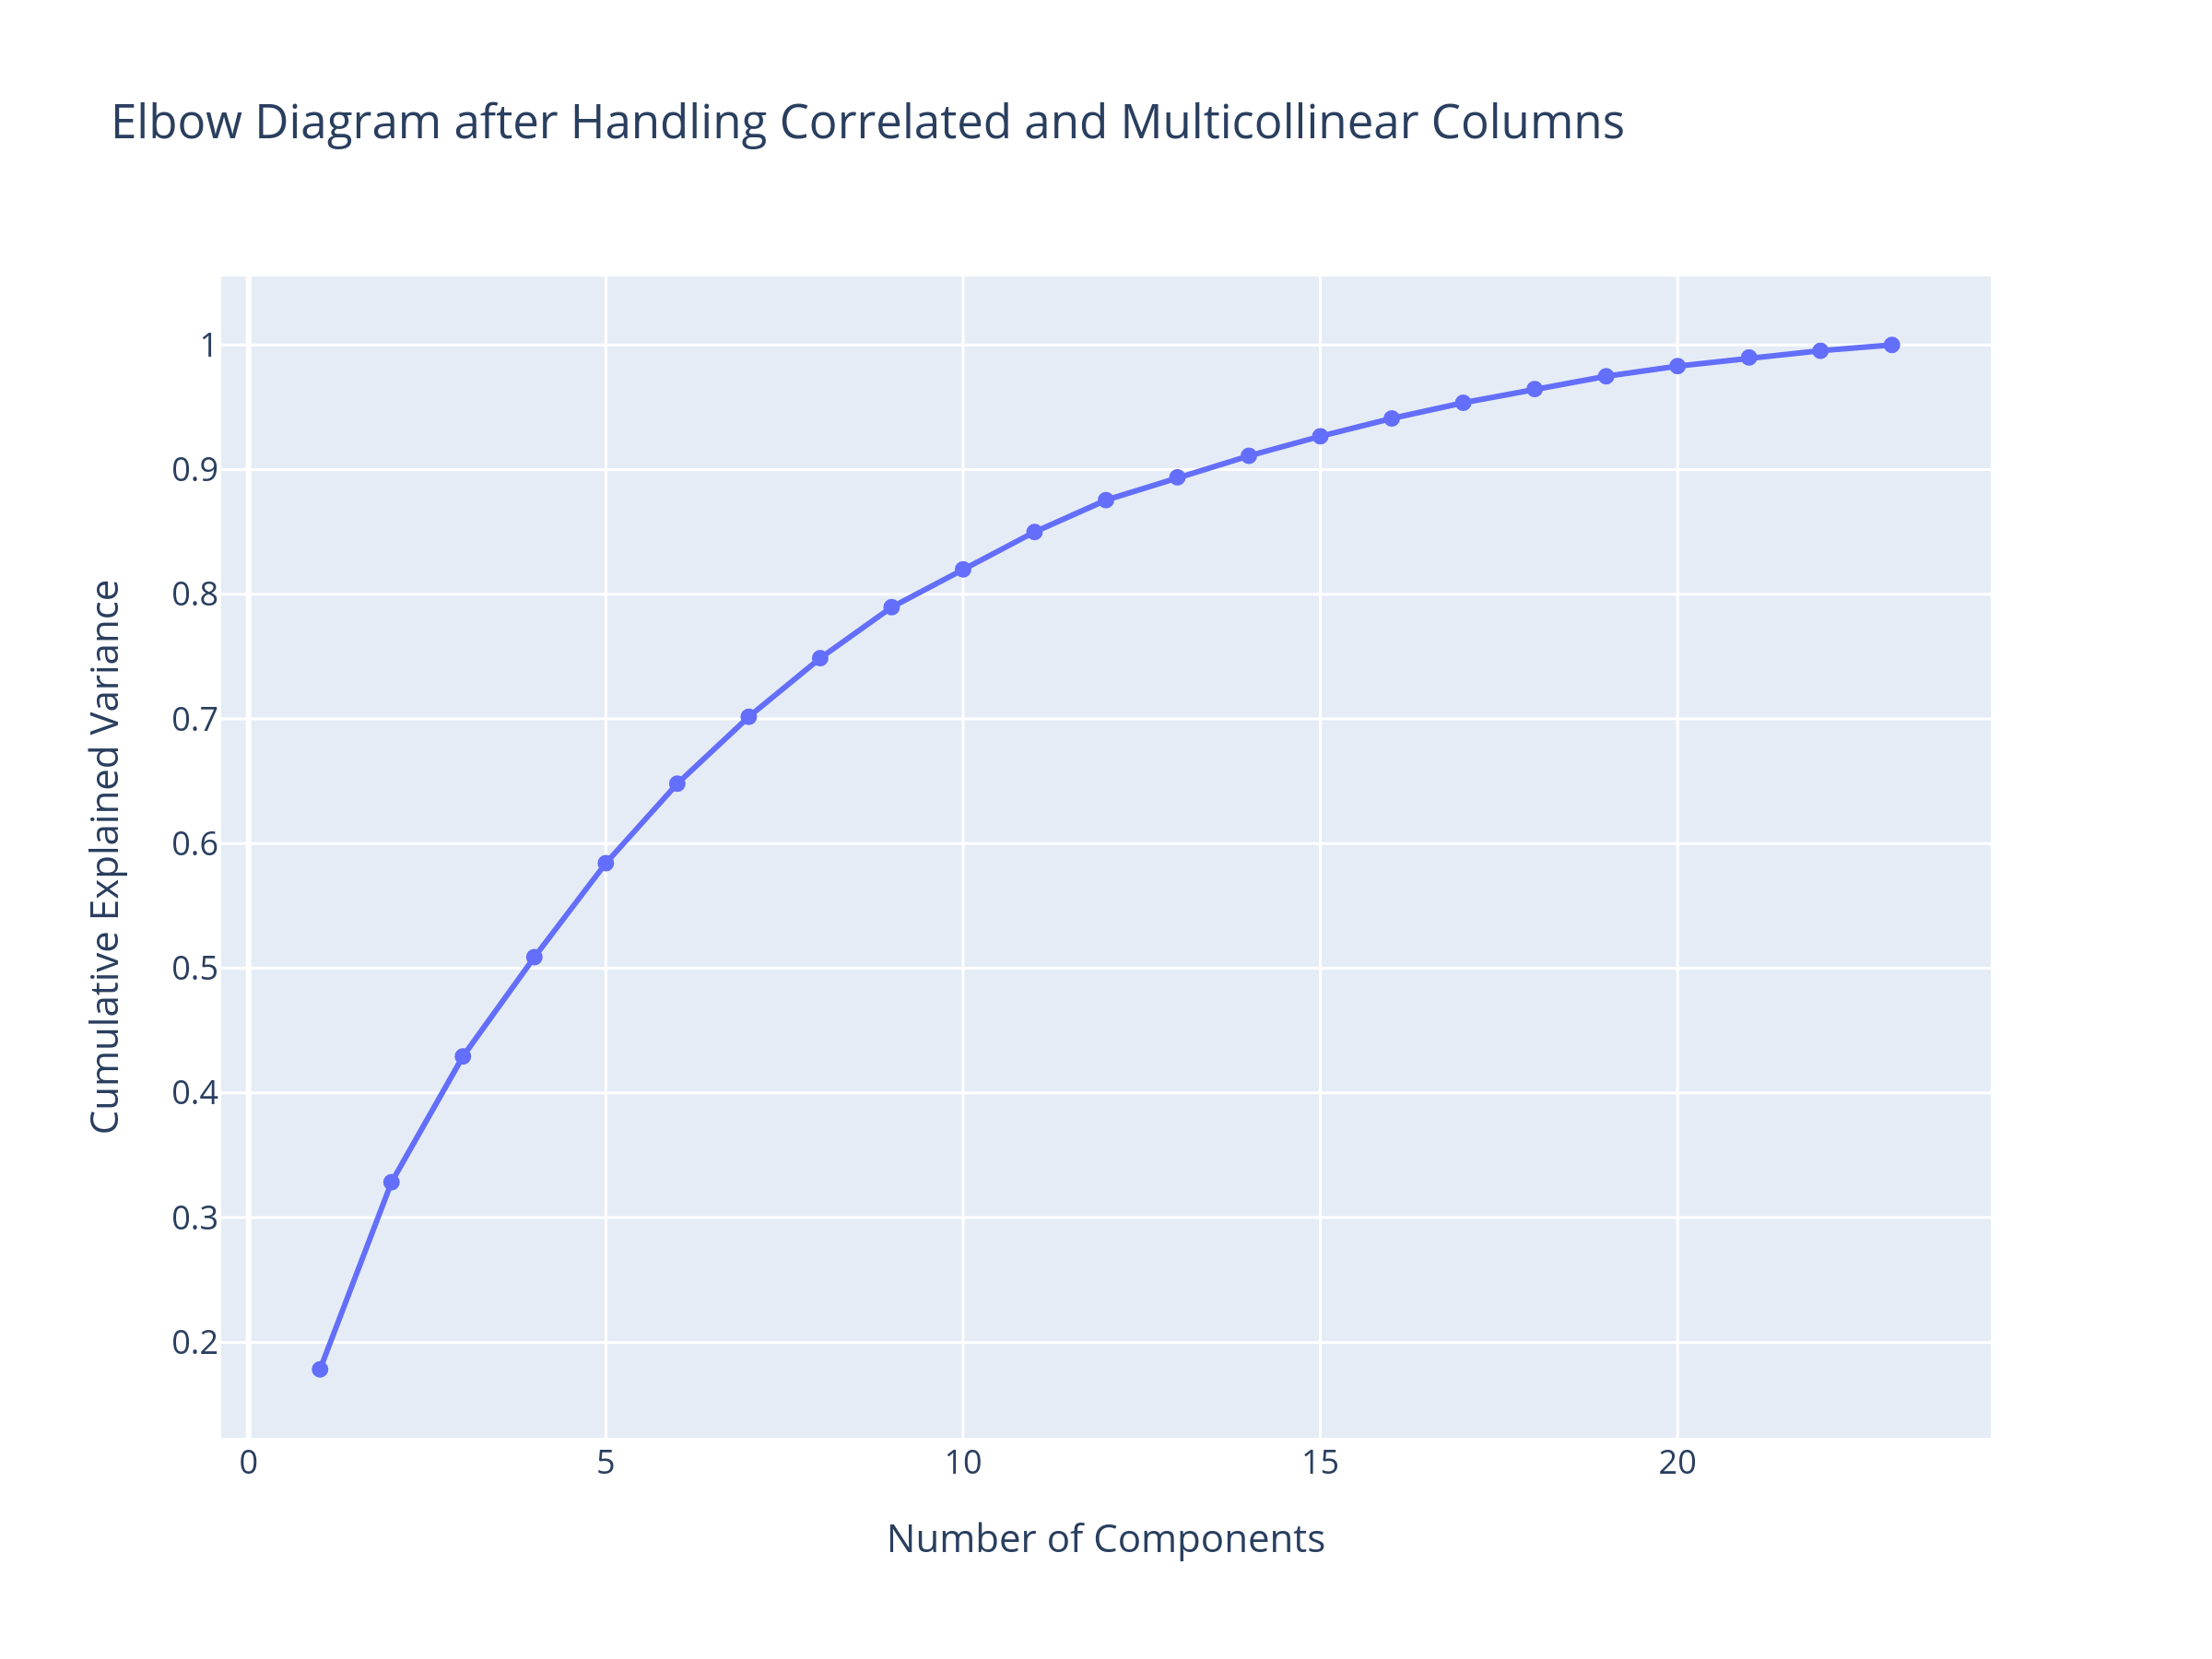
\includegraphics[width=0.6\textwidth]{Images/elbow_diagram_after_vif.png}
    \caption{Elbow Diagram (After Removing Correlated Features)}
\end{figure}

\subsection{Conclusion}
This analysis provided insights into the dataset, with significant findings related to data cleaning, correlation, multicollinearity, and dimensionality reduction through PCA. The methodology applied can be used as a standard approach for similar datasets.

\clearpage